
In order to conduct the multi-strand analysis with the quench velocity-based approach, one should estimate the quench velocity for varying values of magnetic field strength and current that are reached in the magnet. In the previous section, it was concluded that the maximum magnetic field strength in the skew quadrupole equals $B=3~\text{T}$ and occurs at the initial value of current, $I=86~\text{A}$. Therefore, two following main parameters, that have a direct impact on the quench velocity are studied in this section: $(i)$ magnetic field strength, $(ii)$ transport current. In order to conduct the analyses, the standard ANSYS simulations are performed based on 1D models of a relatively short length.

\subsection{Update of Skew Quadrupole Geometry}
\label{subsection:update_skew_quadrupole_geometry}

After preliminary study of the quench propagation in the modelled coil, the modelling of an insulated strand is reformulated in this chapter. The new model aims at parametrising the influence of resin on the heat capacity of the coil. The actual volume of resin between the windings remains an open question from the design standpoint. In the fabrication process, the insulated strand is wound first and the resin is added later to the pre-assembled coil. Therefore, including the resin volume in LINK33 elements is a too conservative assumption leading to a relatively slow turn-to-turn propagation. Therefore, the heat capacity of resin is optionally added with MASS71 elements.

Figure~\ref{fig: 1d_strand_geometry_with_heat_capacity} presents a new 1D+1D model representing a three-dimensional strand. In the~right picture, the nodes marked in red are modelled with the LINK33 element and the strand marked in yellow -- with LINK68. The blue points represent MASS71 elements including an~additional heat capacity in the strand. MASS71 is a point element with temperature as a degree of freedom characterised by a negligible thermal resistance~\cite{ansys_element_manual}. LINK68 has the material properties of the composite strand whereas both LINK33 and MASS71 -- of G10. The main reason for a change is that, in reality, the external insulation layers are in direct contact (marked in red in the left picture of Fig.~\ref{fig: 1d_strand_geometry_with_heat_capacity}) omitting the resin (marked in blue in the left picture of Fig.~\ref{fig: 1d_strand_geometry_with_heat_capacity}). 

\begin{figure}[H]
    \centering
    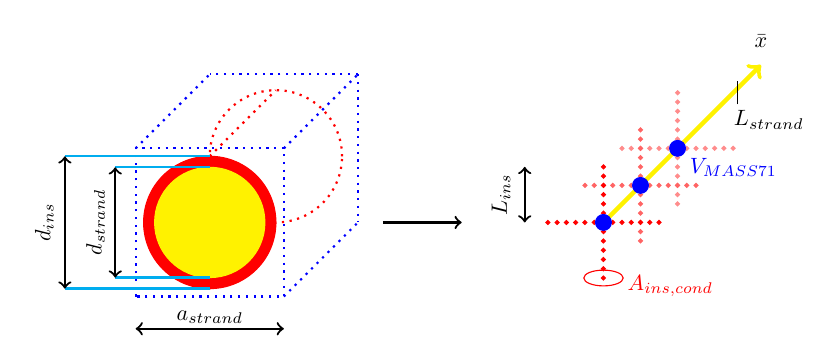
\begin{tikzpicture}[scale = 1]
    
        \draw[thick, blue, dotted] (-0.941,-0.941) rectangle (0.941,0.941);
        \draw[thick, red, dotted] (0.84,0.84) circle (0.7+0.07*2);
        \draw[thick, dotted, red] (0,0.84) -- (0.84,2*0.84);
        \draw[thick, dotted, red] (0,-0.84) -- (0.84,0);
    
        \filldraw[red] (0,0) circle (0.7+0.07*2);
        \filldraw[yellow] (0,0) circle (0.7);
        \draw[thick, cyan] (-0.8*1.5,0.7) -- (0,0.7);
        \draw[thick, cyan] (-0.8*1.5,-0.7) -- (0,-0.7);
        \draw[black, thick, <->] (-0.75*1.6,0.7) -- (-0.75*1.6,-0.7);
        \node[scale = 0.8, rotate=90] at (-1.45, 0) {$d_\text{strand}$};
        
        \draw[thick, cyan] (-0.8*2.3,0.84) -- (0,0.84);
        \draw[thick, cyan] (-0.8*2.3,-0.84) -- (0,-0.84);
        \draw[black, thick, <->] (-0.8*2.3,0.84) -- (-0.8*2.3,-0.84);
        \node[scale = 0.8, rotate=90] at (-2.1, 0) {$d_\text{ins}$};
        \draw[thick, dotted, blue] (0.941,0.941) -- (2*0.941,2*0.941);
        \draw[thick, dotted, blue] (-0.941,0.941) -- (0,2*0.941);
        \draw[thick, dotted, blue] (0.941,-0.941) -- (2*0.941,0);
        \draw[thick, dotted, blue] (2*0.941,2*0.941) -- (2*0.941,0);
        \draw[thick, dotted, blue] (2*0.941,2*0.941) -- (0,2*0.941);

        \node[scale = 0.8] at (0, -1.2) {$a_\text{strand}$};
        \draw[thick,<->] (-0.941,-0.9*1.5) -- (0.941,-0.9*1.5);
        
        % ellipse for insulation area
        \draw[red] (5.0,-5.646/8) ellipse (0.25cm and 0.1cm);
        \node[scale = 0.8, red] at (5.85, -5.646/8-0.1) {$A_\text{ins,cond}$};
        % third insulation layer
        \definecolor{red_third_layer}{RGB}{255,140,140}
        \foreach \x in {-5.646,-4.705,...,5.646} 
            \filldraw[red_third_layer] (5.0+2*0.4705,\x/8+2*0.4705) circle (0.025);
        \foreach \x in {-5.646,-4.705,...,5.646} 
            \filldraw[red_third_layer] (5.0+\x/8+2*0.4705,2*0.4705) circle (0.025);
        % second insulation layer
        \definecolor{red_second_layer}{RGB}{255,100,100}
        \foreach \x in {-5.646,-4.705,...,5.646} 
            \filldraw[red_second_layer] (5.0+0.4705,\x/8+0.4705) circle (0.025);
        \foreach \x in {-5.646,-4.705,...,5.646} 
            \filldraw[red_second_layer] (5.0+\x/8+0.4705,0.4705) circle (0.025);
        % first insulation layer
        \definecolor{red_first_layer}{RGB}{255,0,0}
        \foreach \x in {-5.646,-4.705,...,5.646} 
            \filldraw[red_first_layer] (5.0,\x/8) circle (0.025);
        \foreach \x in {-5.646,-4.705,...,5.646} 
            \filldraw[red_first_layer] (5.0+\x/8,0) circle (0.025);
        % strand nodes
        \draw[ultra thick, yellow, ->] (5.0,0) -- (7.0,2.0);
        \foreach \t in {0.0,0.4705,...,1.4115}
            \filldraw[blue] (5.0+\t,\t) circle (0.1);
        \node[scale = 0.8] at (7.1, 1.3) {$L_\text{strand}$};    
        \node[scale = 0.8] at (7, 2.3) {$\bar x$};    
        \draw[thin] (6.7,1.5) -- (6.7,1.8);
        \draw[thick, black, <->] (4,0) -- (4,5.646/8);
        \node[scale = 0.8, rotate=90] at (3.7, 5.646/16) {$L_\text{ins}$}; 
        % draw arrow
        \draw[thick, black, ->] (2.2,0) -- (3.2,0);
        
        \node[blue, scale = 0.8] at (6.65, 0.7) {$V_\text{MASS71}$}; 
        
    \end{tikzpicture}
    \caption{3-dimensional transformation of a 1D+1D strand domain in ANSYS.}
    \label{fig: 1d_strand_geometry_with_heat_capacity}
\end{figure}


This time, the insulation cross-sectional area $A_\text{ins}$ only takes into account the external insulation layer marked in red as
\begin{equation}
    A_\text{ins} = \frac{\pi}{4} \left( d^2_\text{ins} - d^2_\text{strand} \right),
    \label{eqn:new_cross_sectional_area_insulation}
\end{equation}
where $d_\text{ins}$ -- strand diameter with insulation, $d_\text{strand}$ -- strand diameter. Then, the average perimeter is calculated as
\begin{equation}
    p_\text{avg} =  \frac{\pi}{2} \left( d_\text{ins} + d_\text{strand} \right).
    \label{eqn:new_average_perimeter}
\end{equation}
By combining (\ref{eqn:new_cross_sectional_area_insulation}) and (\ref{eqn:new_average_perimeter}) with (\ref{eqn:equivalent_insulation_length}) one can obtain an equivalent insulation length $L_\text{ins}$. The conduction area $A_\text{ins, cond}$ is calculated as 
\begin{equation}
    A_\text{ins, cond} = \frac{1}{4}~\frac{ A_\text{ins} ~ L_{winding}}{L_\text{ins}}~\frac{1}{n_\text{divisions, winding}}~u_\text{ins},
    \label{eqn:new_equivalent_insulation_element_area}
\end{equation}
where $n_\text{divisions, winding}$ -- number of divisions applied along the winding, $u_\text{ins}$ -- coefficient of the insulation area, $L_\text{winding}$ -- straight winding length of the coil calculated as
\begin{equation}
    L_\text{winding} = 2~(d+e),
\end{equation}
where the parameters $d$ and $e$ are presented in Fig.~\ref{fig: winding_length_in_skew_quad}. The curvature lengths are not taken into account because they vary with an increasing number of a winding layer.

\begin{figure}[H]
    \centering
    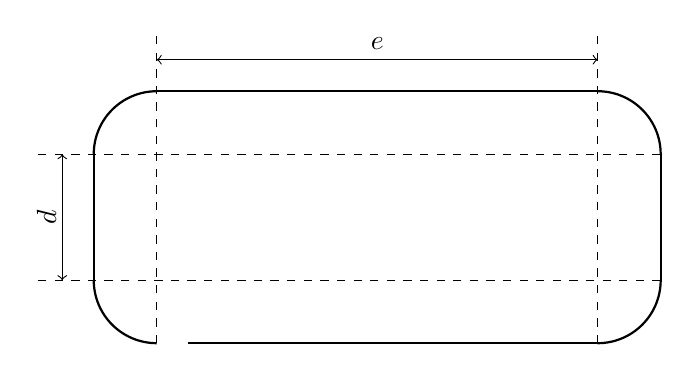
\begin{tikzpicture}[scale = 0.8]
    
        \draw[thick] (0.5,0) -- (7,0);
        \draw[thick] (7,0) arc (-90:0:1);
        \draw[thick] (8,1) -- (8,3);
        \draw[thick] (8,3) arc (0:90:1);
        \draw[thick] (7,4) -- (0,4);
        \draw[thick] (0,4) arc (-270:-180:1);
        \draw[thick] (-1,3) -- (-1,1);
        \draw[thick] (-1,1) arc (-180:-90:1);
        
        \draw[dashed] (0,0) -- (0,5);
        \draw[dashed] (7,0) -- (7,5);
        \draw[dashed] (8,1) -- (-2,1);
        \draw[dashed] (8,3) -- (-2,3);
        
        \draw[<->] (0,4.5) -- (7,4.5);
        \draw[<->] (-1.5,1) -- (-1.5,3);
        
        \node[scale = 1.0] at (3.5,4.75) {$e$};
        \node[scale = 1.0, rotate=90] at (-1.75,2) {$d$};
        
    \end{tikzpicture}
    \caption{Top view of one winding of a high-order corrector geometry.}
    \label{fig: winding_length_in_skew_quad}
\end{figure}

One can observe that Equation~(\ref{eqn:new_equivalent_insulation_element_area}) is similar to (\ref{eqn:equivalent_insulation_element_area}) but without considering $u_\text{ins}$. If $u_\text{ins} = 1$, the entire insulation volume is packed in the LINK33 elements. If $u_\text{ins} < 1$, the remainder of the insulation volume is added to the volume of point MASS71 elements. A reduction of $u_\text{ins}$ serves for limiting the contact area between the neighbouring wires and, thus, the heat transfer across the insulation. The volume of a point MASS71 element is calculated as 
\begin{equation}
    V_\text{MASS71} = \frac{\left( a^2 - \frac{\pi d_\text{ins}^2}{4} \right) L_\text{winding}}{n_\text{nodes, winding}}~u_\text{resin} + L_\text{ins}~A_\text{ins, cond} ~ \left( 1-u_\text{ins} \right),
    \label{eqn:mass71_volume_element}
\end{equation}
where $u_\text{resin}$ -- resin packing coefficient. If $u_\text{resin} = 0$, no resin is taken into account, whereas if $u_\text{resin} = 1$, the entire resin volume is modelled.

\subsection{Quench Velocity Map}

In this section, a set of 16 standard ANSYS simulations with varying magnetic field strength and current is conducted. As presented in Table~\ref{table: quench_velocity_map_input_parameters_geometry}, a 50~cm-long winding is studied. It is important to mention that the winding length $L_\text{winding}$ refers to a straight strand section from Fig.~\ref{fig: 1d_strand_geometry} defined as $L_\text{strand}$. The~model simulates a strand with full insulation without resin. Therefore, $u_\text{ins}=1$ and $u_\text{resin}=0$. The~number of nodes in the longitudinal direction equals $n_\text{nodes, winding}=500$. That corresponds to a mesh size of 1~mm. 20 nodes across the~insulation layer corresponds to a transverse mesh size of 3.5~$\upmu \text{m}$. The mesh size in all dimensions is based on the reference solution of a standard ANSYS simulation with insulation and epoxy resin deduced in Section~\ref{section:quench_velocity_benchmarking_with_insulation_heat_balance}. The mesh size of the insulation elements is smaller in this section, because no resin is considered. Therefore, the model is even more accurate than the one discussed in Section~\ref{section:quench_velocity_benchmarking_with_insulation_heat_balance}.  

\begin{table}[H]
    \caption{Geometry input parameters.} 
    \vspace{-1.em} 
    \fontsize{10}{10}
    \selectfont 
    \renewcommand{\arraystretch}{1.5}
    \begin{center}
        \begin{tabular}{ ccc }  
        \hline
        parameter & value & unit \\
        \hline
        $L_\text{winding}$ & 0.5 & [m] \\ 
        $L_\text{ins}$ & 0.07 & [mm] \\
        $u_\text{ins}$ & 1.0 & [-] \\
        $u_\text{resin}$ & 0.0 & [-] \\
        $n_\text{nodes, winding}$ & 500 & [-] \\ 
        $n_\text{nodes, insulation}$ & 20 & [-] \\
        \hline 
        \end{tabular}
    \end{center}  
     \label{table: quench_velocity_map_input_parameters_geometry} 
 \end{table}

Table~\ref{table: quench_velocity_map_input_parameters} depicts input parameters for the quench velocity study. The initial temperature profile presented in Fig.~\ref{fig: init_gauss_temp_distr_quench_velocity} is calculated based on~(\ref{eqn: gaussian_temp_ic}). The initial temperature $T_\text{init}$ corresponds to the bath temperature of the measured magnet. 

\begin{table}[H]
    \caption{Parameters for the quench velocity study.} 
    \vspace{-1.em} 
    \fontsize{10}{10}
    \selectfont 
    \renewcommand{\arraystretch}{1.5}
    \begin{center}
        \begin{tabular}{ ccc }  
        \hline
        parameter & value & unit \\
        \hline
        $I$ & 26, 46, 66, 86 & [A] \\
        $B$ & 0, 1, 2, 3 & [T] \\
        $T_\text{init}$ & 4.3 & [K] \\
        $T_\text{max}$ & 20.0 & [K] \\
        $L_\text{quench, init}$ & 0.1 & [m] \\ 
        $\alpha$ & 0.223 & [m] \\   
        $t_\text{total}$ & 0.1 & [s] \\
        $t_\text{step range}$ & $[0.01, 0.1]$ & [ms] \\
        \hline 
        \end{tabular}
    \end{center}  
     \label{table: quench_velocity_map_input_parameters} 
 \end{table}

\begin{figure}[H]
\centering
    \begin{tikzpicture}
        \begin{axis}[
          no markers,
          width=0.7\linewidth, 
          height = 4.0cm,
          xlabel={$\bar{x},~\text{m}$},
          ylabel={$T,~\text{K}$},
          xmin=0.0,
          ymin=0.0,
          xmax=0.5,
          xtick= {0,0.1,0.2,0.3,0.4,0.5}
          ]
          \addplot table[x=position,y=temperature,col sep=comma] {sections/skew_quad_q_det/figures/v_quench_map/init_gauss_profile.csv}; 
        \end{axis}
    \end{tikzpicture}
    \caption{Initial Gaussian temperature profile.}
    \label{fig: init_gauss_temp_distr_quench_velocity}
\end{figure}

In the first instants of the quench analysis, the quench velocity is usually higher. However, there is a moment in the simulations when the heat generation predominates the longitudinal heat propagation in the quenched zone. At that moment, the quench velocity stabilises and remains relatively constant. 

The quench velocity is calculated as in~(\ref{eqn:new_quench_velocity}) with a time window equal to $\Delta t=10~\text{ms}$. If the difference in the quench velocity between two consecutive time windows varies less than 0.1~m/s, it is assumed that the quench propagation stabilises. As soon as this condition is met, the analysis finishes and the final value of the quench velocity is saved. Figure~\ref{fig: v_quench_map_current_b_field} presents the quench velocity map as a function of the magnetic field strength and current.

\begin{figure}[H]
\centering
    \begin{tikzpicture}
        \begin{axis}[
          width=0.7\linewidth, 
          height = 4.0cm,
          xlabel={$B$, $\text{T}$},
          ylabel={$v_\text{quench}$, $\frac{\text{m}}{\text{s}}$},
          xmin=0.0,
          xmax=3.0,
          ymin=0.0,
          ymax=6.0,
          legend pos = outer north east
          ]
          \addplot[green, mark=*] table[x=B_field,y=I_86,col sep=comma] {sections/skew_quad_q_det/figures/v_quench_map/v_quench_map.csv};
          \addplot[blue, mark=*] table[x=B_field,y=I_66,col sep=comma] {sections/skew_quad_q_det/figures/v_quench_map/v_quench_map.csv};
          \addplot[red, mark=*] table[x=B_field,y=I_46,col sep=comma] {sections/skew_quad_q_det/figures/v_quench_map/v_quench_map.csv};
          \addplot[black, mark=*] table[x=B_field,y=I_26,col sep=comma] {sections/skew_quad_q_det/figures/v_quench_map/v_quench_map.csv};
          \legend{
          $I=86~\text{A}$,
          $I=66~\text{A}$,
          $I=46~\text{A}$,
          $I=26~\text{A}$}
        \end{axis}
    \end{tikzpicture}
    \caption{Quench velocity map as a function of magnetic field strength and current.}
    \label{fig: v_quench_map_current_b_field}
\end{figure}